% executive_brief.tex -> ../consensus_change_standards_brief_v4.pdf
% A standalone 1-2 page companion to the full paper, for policymakers, operators,
% and time-pressed readers. Every claim is drawn verbatim/faithfully from the
% verified 4th-edition treatise (abstract/§3.4, §5.1-§5.2, §5.4, §4.0). It adds
% nothing to and removes nothing from the 96-page paper.
\documentclass[11pt]{article}
\usepackage[letterpaper, margin=0.85in]{geometry}
\usepackage{mathpazo}
\usepackage[T1]{fontenc}
\usepackage{microtype}
\usepackage{xcolor}
\usepackage{graphicx}
\usepackage{titlesec}
\usepackage{enumitem}
\usepackage[hidelinks]{hyperref}
\usepackage{tcolorbox}

\definecolor{bitcoinorange}{HTML}{F7931A}
\definecolor{navy}{HTML}{0D1117}
\definecolor{chaptergray}{RGB}{80,80,80}
\linespread{1.06}
\setlength{\parindent}{0pt}
\setlength{\parskip}{5pt}
\pagestyle{empty}

\titleformat{\section}{\large\bfseries\color{chaptergray}}{}{0pt}{}
\titlespacing{\section}{0pt}{8pt}{2pt}

\hypersetup{pdftitle={Consensus Change Standards --- Executive Brief (4th ed.)},
  pdfauthor={Asaf Fulks}, pdfsubject={Bitcoin Protocol Governance},
  pdfkeywords={Bitcoin, consensus change, soft fork, BIP, protocol governance, BIP-110, chain split, activation threshold}}

\begin{document}

% ---- masthead ----
{\color{bitcoinorange}\rule{\linewidth}{2pt}}
\vspace{4pt}

{\fontsize{22}{26}\selectfont\bfseries Consensus Change Standards}\\[2pt]
{\large\itshape Executive Brief --- a summary for policymakers, operators, and busy readers}\\[3pt]
{\small A Legal and Technical Framework for Bitcoin Protocol Governance \textbf{·} Fourth Edition, 2026 \textbf{·} The Forum Press}

\vspace{2pt}
{\color{bitcoinorange}\rule{\linewidth}{0.8pt}}

% ---- thesis callout ----
\begin{tcolorbox}[colback=bitcoinorange!7, colframe=bitcoinorange!60, boxrule=0.8pt,
  arc=2.5pt, left=10pt, right=10pt, top=8pt, bottom=8pt, before skip=10pt, after skip=10pt]
{\centering
The catastrophic failure mode of a Bitcoin consensus change\,---\,a permanent chain split\,---\,has a \textbf{computable} probability. At \textbf{55\%} hashrate enforcement the chance of a six-block reorganization during activation is roughly \textbf{thirty percent}; by \textbf{90\%} or above it is \textbf{effectively zero}, five to seven orders of magnitude lower. Much of the governance argument is a fight over that one number.\par}
\end{tcolorbox}

% ---- what this is ----
\section{What this is}
A neutral, public \textbf{20-criterion readiness checklist} for judging whether a proposed change to Bitcoin's shared consensus rules has been adequately reviewed before it goes live. The criteria fall in four groups\,---\,\textbf{Proposal Quality, Code Quality, Activation Safety, Community Process}\,---\,and a proposal is scored Green / Yellow / Orange / Red on the share it meets. It is \textbf{not} a proposed law and \textbf{not} a change to Bitcoin's code; it sets standards for the \emph{process} by which changes are evaluated, debated, and adopted or rejected. It is procedurally neutral\,---\,the same standards apply whether a change would liberalize Bitcoin's policy or restrict it.

% ---- what it found ----
\section{What it found}
\begin{figure}[h]
\centering
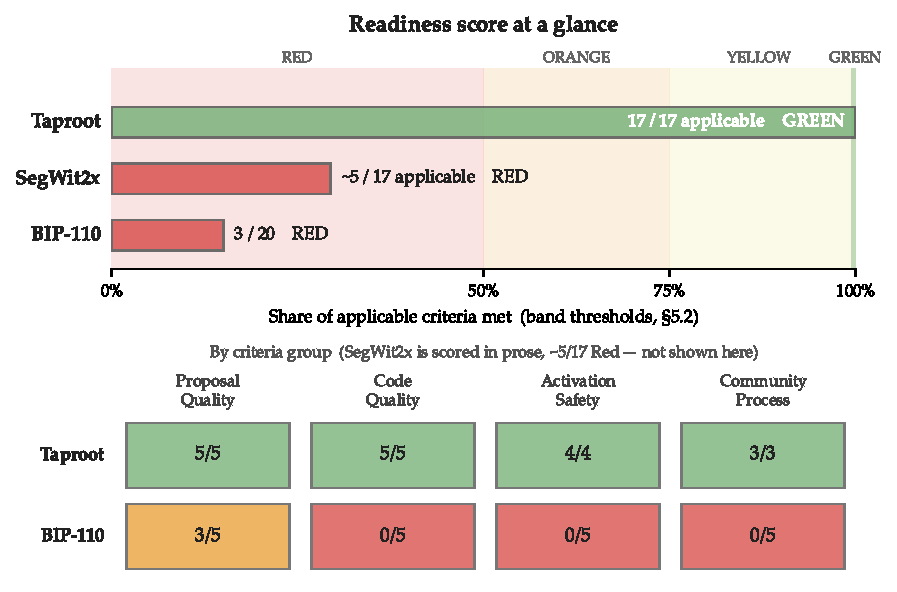
\includegraphics[width=0.92\linewidth]{fig-5-2-scorecard.pdf}
\end{figure}

\vspace{-4pt}
Applied to real proposals: \textbf{Taproot scores 17/17 (Green)}; \textbf{BIP-110 scores 3/20 (Red)}; and \textbf{SegWit2x scores roughly 5/17 (Red)}. To show the framework measures \emph{process, not preference}, it also scores a hypothetical change the author's own mining revenue would favor\,---\,and that change scores Red too.

% ---- legal teeth ----
\section{Why a policymaker should care}
A rushed change that ignores documented red flags is not just a technical risk\,---\,it is a \textbf{legal} one. The framework's force is \textbf{deterrence, not enforcement}: a documented Red score is a dated, public record that supplies the \emph{notice} and \emph{foreseeability} the negligence and negligent-misrepresentation theories of the full paper's legal analysis depend on, should a change be activated anyway and cause loss. The flip side is the protection: \textbf{following the standard is itself the defense.} Compliance is the defense; the score is the exposure.

% ---- not a cartel ----
\section{Is it a cartel?}
No. The framework \textbf{binds no one and asks for no agreement}: it publishes criteria each operator applies \emph{unilaterally} to the listing, custody, and risk decisions it already makes. Independent parallel conduct on published criteria is not a Sherman Act violation; only an actual \emph{agreement} to refuse would raise the antitrust concern\,---\,the posture the framework is designed never to form, and the model adoption language is drafted accordingly.

\vfill
{\color{bitcoinorange}\rule{\linewidth}{0.8pt}}
\vspace{3pt}
{\small\textbf{Read the full 96-page paper.} \href{https://github.com/asaffulks/consensus-change-standards}{\nolinkurl{github.com/asaffulks/consensus-change-standards}} \textbf{·} DOI \texttt{10.5281/zenodo.20651832} \textbf{·} \textit{Cite as:} Asaf Fulks, \textit{Consensus Change Standards: A Legal and Technical Framework for Bitcoin Protocol Governance} (4th ed.~2026). This brief summarizes; the paper, its authorities, and its caveats govern.}

\end{document}
